% THIS DOCUMENT IS TAILORED TO REQUIREMENTS FOR SCIENTIFIC COMPUTING.  IT SHOULDN'T
% BE USED FOR NON-SCIENTIFIC COMPUTING PROJECTS
\documentclass[12pt]{article}

\usepackage{amsmath, mathtools}
\usepackage{amsfonts}
\usepackage{amssymb}
\usepackage{graphicx}
\usepackage{caption}
\usepackage{colortbl}
\usepackage{xr}
\usepackage{hyperref}
\usepackage{longtable}
\usepackage{xfrac}
\usepackage{tabularx}
\usepackage{float}
\usepackage{siunitx}
\usepackage{booktabs}
\usepackage{caption}
\usepackage{pdflscape}
\usepackage{afterpage}
\usepackage{cite}

%\usepackage{refcheck}

\hypersetup{
    bookmarks=true,         % show bookmarks bar?
      colorlinks=true,       % false: boxed links; true: colored links
    linkcolor=red,          % color of internal links (change box color with linkbordercolor)
    citecolor=green,        % color of links to bibliography
    filecolor=magenta,      % color of file links
    urlcolor=cyan           % color of external links
}

%% Comments

\usepackage{color}

\newif\ifcomments\commentstrue %displays comments
%\newif\ifcomments\commentsfalse %so that comments do not display

\ifcomments
\newcommand{\authornote}[3]{\textcolor{#1}{[#3 ---#2]}}
\newcommand{\todo}[1]{\textcolor{red}{[TODO: #1]}}
\else
\newcommand{\authornote}[3]{}
\newcommand{\todo}[1]{}
\fi

\newcommand{\wss}[1]{\authornote{magenta}{SS}{#1}} 
\newcommand{\plt}[1]{\authornote{cyan}{TPLT}{#1}} %For explanation of the template
\newcommand{\an}[1]{\authornote{cyan}{Author}{#1}}

%% Common Parts

\newcommand{\progname}{Software Engineering} 
\newcommand{\authname}{Team \#6, Six Sense
\\ Omar Alam
\\ Sathurshan Arulmohan
\\ Nirmal Chaudhari
\\ Kalp Shah
\\ Jay Sharma
}        

\usepackage{hyperref}
    \hypersetup{colorlinks=true, linkcolor=blue, citecolor=blue, filecolor=blue,
                urlcolor=blue, unicode=false}
    \urlstyle{same}
                                


% For easy change of table widths
\newcommand{\colZwidth}{1.0\textwidth}
\newcommand{\colAwidth}{0.13\textwidth}
\newcommand{\colBwidth}{0.82\textwidth}
\newcommand{\colCwidth}{0.1\textwidth}
\newcommand{\colDwidth}{0.05\textwidth}
\newcommand{\colEwidth}{0.8\textwidth}
\newcommand{\colFwidth}{0.17\textwidth}
\newcommand{\colGwidth}{0.5\textwidth}
\newcommand{\colHwidth}{0.28\textwidth}

% Numbering 
\usepackage{amsthm}
\usepackage{xassoccnt}
%\newtheorem{req}{Requirement}[section]        
\newtheorem{req}{Requirement}        
\theoremstyle{definition}        
\newtheorem{constraint}{Constraint}
\newtheorem{goal}{Goal}
\DeclareCoupledCountersGroup{theorems}
\DeclareCoupledCounters[name=theorems]{req,constraint,goal}
\setcounter{goal}{0}

\usepackage{fullpage}


\begin{document}

\title{Software Requirements Specification for \progname: subtitle describing software} 
\author{\authname}
\date{\today}
	
\maketitle

~\newpage

\pagenumbering{roman}

\tableofcontents

~\newpage

\section*{Revision History}


\begin{tabularx}{\textwidth}{p{3cm}p{2cm}X}
\toprule {\bf Date} & {\bf Version} & {\bf Notes}\\
\midrule
2025-10-06 & 1.0 & Initial Write-up\\
\bottomrule
\end{tabularx}


~\newpage

\section{Goal}

\subsection{G.1 Context and overall objective}

With around 4 million Canadians affected by hearing loss \cite{Healthing2025}, 
there is a significant need for assistive technologies that can improve 
situational awareness and safety.
Many safety cues and general sound alerts such as the sound of a car 
approaching, a kettle whistling,
or a phone ringing may be missed, leading to increased risk of injury and
miscommunication.

Many existing solutions focus on speech transcription, but lack the ability to
provide directional information about sound sources or classify non-speech
sounds. This project aims to address this gap by developing an assistive device
that provides real-time visual indications of sound source locations and 
classifications.

The objective of this project is to develop an assistive device that aids
individuals who are deaf or hard of hearing by providing real-time visual
indications of sound source locations and classifications (ex. 'car on your 
left').

Some of the high-level goals of the project are:

\begin{goal}\label{goal:audio_capture}
Capture real-time audio data from a 
\hyperref[def:microphone_array]{microphone array}
with synchronized sampling to enable accurate situational analysis
of sound sources.
\end{goal}

\begin{goal}\label{goal:audio_direction_analysis}
Analyze captured audio to determine the direction of arrival (DoA) of
sound sources with minimal error and with minimal latency nearing real-time.
\end{goal}

\begin{goal}\label{goal:audio_identification_analysis}
Analyze captured audio to classify the sound sources with their English
label (ex. 'car', 'phone', 'kettle', 'alarm', 'speech').
\end{goal}

\begin{goal}\label{goal:visual_display}
Display audio classification and transcription on smart glasses in real-time
without obstructing the user's field of view.
\end{goal}

\begin{goal}\label{goal:user_friendly_interaction}
Provide a user-friendly interaction with the smart glasses,
allowing the user to easily set up, use, and understand visual indicators.
\end{goal}

\begin{goal}\label{goal:user_comfort}
Ensure that the system is comfortable to wear for extended periods of time,
with minimal discomfort or fatigue.
\end{goal}
    
\subsection{G.2 Current situation}

Currently, individuals who are deaf or hard of hearing face significant
challenges in maintaining situational awareness due to missed audio cues.
Existing assistive technologies address some aspects of this problem, but
leave critical gaps:

\begin{itemize}
\item \textbf{Smart glasses with transcription capabilities:} Some devices
can listen to live human audio and transcribe it to text (multilingual) in
real-time, displaying the transcript on a smartphone display.
However, these solutions focus solely on speech transcription and do not
provide directional information about sound sources or classify non-speech
sounds.

\item \textbf{Hearing aids:} Traditional hearing aids amplify ambient sounds
to improve awareness of audio sources at various volumes \cite{NIDCD2022}. 
While this helps individuals with partial hearing loss, it does not assist 
those who are profoundly deaf, nor does it provide visual cues about sound 
direction or classification.

\item \textbf{Notification systems:} Some home automation systems can send
visual alerts (e.g., flashing lights) when specific sounds are detected,
such as doorbells or smoke alarms. However, these systems are limited to
fixed locations and predetermined sound types, lacking portability and
real-time directional awareness.
\end{itemize}

The current solutions fail to address the critical need for real-time,
portable, directional awareness of environmental sounds, leaving individuals
vulnerable to missing important safety cues such as approaching vehicles,
warning beeps from machinery, or emergency alerts.

\subsection{G.3 Expected benefits}

The proposed system will deliver significant improvements to the daily lives
and safety of individuals who are deaf or hard of hearing:

\begin{itemize}
\item \textbf{Real-time spatial awareness:} Enable identification of sound
source locations on a 2D plane in real-time, allowing users to quickly
orient themselves toward important sounds such as someone calling their name,
an approaching vehicle, or an emergency alarm.

\item \textbf{Enhanced safety:} Reduce the risk of injury by alerting users
to critical safety cues that are typically communicated through sound, such
as warning beeps from forklifts, tea kettles whistling, car engines
or emergency sirens (from emergency vehicles) approaching from behind.

\item \textbf{Improved situational awareness:} Provide continuous awareness
of the acoustic environment without requiring the user to constantly scan
their surroundings, reducing cognitive load and enabling more natural
interactions with their environment.

\item \textbf{Sound classification:} Differentiate between various types of
sounds (e.g., speech, alarms, vehicles, household appliances) to help users
prioritize their attention and responses appropriately.

\item \textbf{Reduced frustration and miscommunication:} Minimize instances
of missed phone calls, doorbell rings, or verbal attempts to gain the user's
attention, leading to smoother social interactions and reduced social
isolation.

\item \textbf{Portable and wearable solution:} Unlike fixed home automation
systems, the smart glasses form factor provides continuous protection and
awareness regardless of location, whether at home, work, or in public spaces.

\item \textbf{Independence and confidence:} Empower users to navigate their
environment more independently without relying on others to alert them to
important sounds, fostering greater autonomy in daily activities.
\end{itemize}



\subsection{G.4 Functionality overview}

The system will provide the following principal functions:

\begin{itemize}
\item \textbf{Real-time audio capture:} Continuously capture audio signals
from a synchronized microphone array mounted on smart glasses, ensuring
precise temporal alignment for accurate spatial analysis.

\item \textbf{Direction of arrival (DoA) estimation:} Process captured audio
to determine the angular direction of sound sources on a 2D plane relative
to the user's position, with a target accuracy of ±45° for single sound
sources.

\item \textbf{Sound source classification:} Analyze audio characteristics to
classify detected sounds into meaningful categories (e.g., speech, vehicle
sounds, alarms, household appliances) using audio fingerprinting techniques,
with a target accuracy of at least 90\%.

\item \textbf{Visual feedback generation:} Generate intuitive visual
representations of detected sound sources, including their direction and
classification, displayed on the smart glasses interface with minimal
latency ($\leq$1 second).

\item \textbf{Multi-source handling:} Detect and track multiple simultaneous
sound sources when feasible, prioritizing the most relevant or critical
sounds based on classification and proximity.

\item \textbf{Real-time processing:} Execute all signal processing,
direction estimation and classification algorithms real-time,
with consistent performance and low latency.

\item \textbf{Noise cancellation or audio filtering:} The system will
modify or filter the actual sounds in the environment based on direction
of arrival in order to improve directional hearing. This would help improve
the quality of the transcriptions provided by the system.
\end{itemize}

\subsection{G.5 High-level usage scenarios}

The following scenarios illustrate fundamental usage paths through the system:

\subsubsection{Scenario 1: Pedestrian crossing detection}
A user is walking in an urban environment and approaches a street
intersection. As they prepare to cross, a car approaches from their left
side. The system detects the engine sound, estimates its direction (e.g.,
90° to the left), classifies it as a vehicle, and displays a visual
indicator on the smart glasses showing the direction and classification.
The user recognizes the alert and waits for the vehicle to pass before
crossing safely.

\subsubsection{Scenario 2: Kitchen safety alert}
A user is cooking in their kitchen when a tea kettle on the stove begins
to whistle. The system captures the high-pitched sound through the
microphone array, determines that it is coming from behind and to the
right (e.g., 135°), classifies it as a kettle or alarm sound, and displays
a directional indicator. The user turns toward the alert and removes the
kettle from heat, preventing a potential hazard.

\subsubsection{Scenario 3: Social interaction}
A user is in a crowded room when someone calls their name from across the
space. The system detects the speech sound, estimates the direction (e.g.,
30° to the right), classifies it as speech or a human voice, and displays
the information on the glasses. The user turns in the indicated direction
to make eye contact and engage in conversation, reducing social friction
and missed interactions.

\subsubsection{Scenario 4: Workplace awareness}
A user is working in an industrial setting when a forklift begins reversing
nearby, emitting a warning beep. The system detects the beeping pattern,
determines its direction (e.g., directly behind at 180°), classifies it as
a warning signal, and alerts the user with a prominent visual indicator.
The user steps aside to maintain a safe distance from the moving equipment.

\subsection{G.6 Limitations and exclusions}

The following aspects are explicitly outside the scope of this project:

\begin{itemize}
\item \textbf{Autonomous danger assessment:} The system will not independently
evaluate whether a detected sound represents an immediate danger or
automatically alert the user of hazardous situations. It will present
directional and classification information, leaving interpretation and
response decisions to the user.

\item \textbf{Augmented reality overlay:} The system will not provide
full augmented reality capabilities with spatial overlays showing sound
locations directly mapped onto the user's field of view. Visual feedback
will be presented through a simpler display interface on the smart glasses.

\item \textbf{User response monitoring:} The system will not track whether
the user has noticed, acknowledged, or responded to presented alerts. There
is no feedback loop to ensure user reaction or to escalate notifications.

\item \textbf{Multilingual speech transcription:} Audio transcription
functionality, if implemented, will be limited to English only. Support
for other languages is not included in the current scope.

\item \textbf{3D spatial localization:} Direction estimation will be
constrained to a 2D horizontal plane around the user. Elevation angle
determination (above or below the user's head level) is excluded from
the core functionality.

\item \textbf{Sound source distance estimation:} While direction will be
provided, the system will not attempt to estimate the absolute distance
to sound sources.

\item \textbf{Continuous recording or data storage:} The system will not
record or store audio data beyond what is necessary for real-time processing.
No historical logs of detected sounds will be maintained.

\item \textbf{Network connectivity:} All processing will
occur locally on the embedded hardware. The system will not require internet
connectivity or cloud-based services for core functionality.
\end{itemize}

\subsection{G.7 Stakeholders and requirements sources}

\subsubsection{Primary stakeholders}

\begin{itemize}
\item \textbf{Individuals who are deaf or hard of hearing:} The primary
end-users of the system, who will directly benefit from improved
situational awareness and safety. This group is quite large in population,
with approximately 4 million people who experience hearing loss 
in Canada alone (1 in 10).
\end{itemize}

\subsubsection{Secondary stakeholders}

\begin{itemize}
\item \textbf{Family members and caregivers:} Individuals who support people
with hearing loss and will benefit from improved communication and reduced
safety concerns.

\item \textbf{Employers and workplace safety officers:} Organizations that
employ individuals with hearing loss and are responsible for maintaining
safe working environments.

\item \textbf{Accessibility advocates and organizations:} Groups focused on
improving quality of life and independence for individuals with disabilities.

\item \textbf{Healthcare providers and audiologists:} Professionals who may
recommend or integrate such assistive technologies into patient care plans.

\item \textbf{Future developers and researchers:} The broader engineering
and scientific community who may build upon this work or apply similar
techniques to related problems.
\end{itemize}

\subsubsection{Requirements sources}

\begin{itemize}
\item \textbf{Academic literature:} Research on hearing loss impact,
assistive technologies, direction of arrival algorithms, and audio
classification techniques.

\item \textbf{Domain experts:}\label{itm:domain-experts} Consultation with domain experts, such as 
Dr. Mohrenschildt, for technical feasibility and requirements validation.

\item \textbf{Existing assistive technologies:} Analysis of current solutions
such as hearing aids, transcription glasses, and home alert systems to
identify gaps and opportunities.

\item \textbf{Hardware and software documentation:} Technical specifications
for microcontroller, source code libraries, smart glasses hardware,
and microphone array components.

\item \textbf{Standards and best practices:} IEEE standards for embedded
systems, accessibility guidelines, and real-time system design principles.

\item \textbf{Proof of concept testing:} Empirical results from prototyping
and laboratory testing to validate technical approaches and refine
requirements.
\end{itemize}


\section{Environment}

\subsection{E.1 Glossary}

\textbf{Microphone Array:}\label{def:microphone_array} A collection of 
microphones that are synchronized to capture audio from the 
environment to create a single multi-channel audio signal.

\subsection{E.2 Components}
\wss{List of elements of the environment that may affect or be affected by the system and project. Includes other systems to which the system must be interfaced.}

\subsection{E.3 Constraints}
\wss{Obligations and limits imposed on the project and system by the environment.}

\subsection{E.4 Assumptions}
\wss{Properties of the environment that may be assumed, with the goal of facilitating the project and simplifying the system.}

\subsection{E.5 Effects}
\wss{Elements and properties of the environment that the system will affect.}

\subsection{E.6 Invariants}
\wss{Properties of the environment that the system’s operation must preserve.}

\section{System}

\subsection{S.1 Components}
\wss{Overall structure expressed by the list of major software and, if applicable, hardware parts.}

\subsection{S.2 Functionality}
\wss{One section, S.2.n, for each of the components identified in S.2, describing the corresponding behaviors (functional and non-functional properties).}

\subsection{S.3 Interfaces}
\wss{How the system makes the functionality of S.2 available to the rest of the world, particularly user interfaces and program interfaces (APIs).}

\subsection{S.4 Detailed usage scenarios}
\wss{Examples of interaction between the environment (or human users) and the system: use cases, user stories.}

This section provides detailed versions of the high-level scenarios from \ref{item:G.5}, with specific technical details and interaction flows.

\subsubsection{S.4.1 Pedestrian Crossing Detection}
\textbf{User Story:} As a deaf individual, I want to be alerted when vehicles are approaching so I can cross streets safely.

\textbf{Scenario:} A user is walking in an urban environment and approaches a street intersection. As they prepare to cross, a car approaches from their left side.

\textbf{Interaction Flow:}
\begin{enumerate}
    \item System detects engine sound pattern characteristic of a vehicle
    \item DoA algorithm estimates direction
    \item Audio classification identifies the sound as a vehicle
    \item Smart glasses display visual indicator showing direction and notifies the user of a vehicle approaching
    \item User recognizes the alert and waits for the vehicle to pass before crossing safely
\end{enumerate}

\subsubsection{S.4.2 Kitchen Safety Alert}
\textbf{User Story:} As a deaf individual, I want to be notified of household safety sounds so I can respond to potential hazards.

\textbf{Scenario:} A user is cooking in their kitchen when a tea kettle on the stove begins to whistle.

\textbf{Interaction Flow:}
\begin{enumerate}
    \item Microphone array captures the high-pitched whistle sound
    \item System processes the audio and identifies the characteristic pattern
    \item DoA algorithm estimates the direction
    \item Audio classification identifies it as a kettle or alarm sound (90\% accuracy target)
    \item Smart glasses display directional indicator notifying the user of a kettle whistling ($\leq 1$s latency)
    \item User turns toward the alert and removes the kettle from heat, preventing potential hazard
\end{enumerate}

\subsubsection{S.4.3 Social Interaction}
\textbf{User Story:} As a deaf individual, I want to know when someone is trying to get my attention so I don't miss social interactions.

\textbf{Scenario:} A user is in a crowded room when someone calls their name from across the space.

\textbf{Interaction Flow:}
\begin{enumerate}
    \item System captures audio from all directions through the microphone array
    \item Voice activity detection identifies human speech patterns
    \item DoA algorithm estimates the direction
    \item Audio classification identifies the sound as speech or human voice
    \item Smart glasses display the information with directional arrow
    \item User turns in the indicated direction to make eye contact and engage in conversation
\end{enumerate}

\subsubsection{S.4.4 Workplace Awareness}
\textbf{User Story:} As a deaf worker, I want to be aware of industrial safety warnings so I can maintain workplace safety.

\textbf{Scenario:} A user is working in an industrial setting when a forklift begins reversing nearby, emitting a warning beep.

\textbf{Interaction Flow:}
\begin{enumerate}
    \item System detects the characteristic beeping pattern through microphone array
    \item DoA algorithm estimates the direction
    \item Audio classification identifies it as a warning signal or industrial alarm
    \item Smart glasses display prominent visual indicator notifying the user of a forklift backing up and directional arrow
    \item User steps aside to maintain a safe distance from the moving equipment
\end{enumerate}

\subsection{S.5 Prioritization}
\wss{Classification of the behaviors, interfaces and scenarios (S.2, S.3 and S.4) by their degree of criticality.}

\subsection{S.6 Verification and acceptance criteria}
\wss{Specification of the conditions under which an implementation will be deemed satisfactory.}

\section{Project}

\subsection{P.1 Roles and personnel}
\wss{Main responsibilities in the project; required project staff and their needed qualifications.}

\subsection{P.2 Imposed technical choices}
\wss{Any a priori choices binding the project to specific tools, hardware, languages or other technical parameters.}

\subsection{P.3 Schedule and milestones}
\wss{List of tasks to be carried out and their scheduling.}

\subsection{P.4 Tasks and deliverables}
\wss{Details of individual tasks listed under P.3 and their expected outcomes.}

\subsection{P.5 Required technology elements}
\wss{External systems, hardware and software, expected to be necessary for building the system.}

\subsection{P.6 Risks and mitigation analysis}
\wss{Potential obstacles to meeting the schedule of P.4, and measures for adapting the plan if they do arise.}

\subsection{P.7 Requirements process and report}
The development of this project requires iterating over various stages of the
requirements process. These stages include:

\begin{enumerate}
    \item \textbf{Elicitation}
    \begin{enumerate}
        \item Conduct stakeholder interviews and surveys to gather users' needs.

        \item Review background documents and research articles describing how
        core features have been implemented in the past.

        \item Consult with the technical supervisor of this application
        (\hyperref[itm:domain-experts]{MVM}) to gain insight into what
        approaches can be used. 
    \end{enumerate}

    \item \textbf{Analysis}
    \begin{enumerate}
        \item Based on information retrieved from the elicitation process,
        derive a list of soft and hard goals for the application.

        \item Using the goals defined previously, derive a list of key
        requirements. This will be influenced by the goals of the stakeholders,
        but also input on potential limitations based on discussion with the
        supervisor.

        \item Group requirements into functional vs.\ non-functional categories.

        \item Prioritize requirements using the MoSCoW framework (Must, Should,
        Could, Won't).

        \item Iteratively evaluate defined requirements based on new constraints
        that arise during implementation. 
    \end{enumerate}

    \item \textbf{Documentation}
    \begin{enumerate}
        \item Write requirements in a structured format that is clear, testable,
        and unambiguous.

        \item Use labels for different requirements and goals for traceability. 
    \end{enumerate}

    \item \textbf{Specification}
    \begin{enumerate}
        \item Using the \texttt{docs/} folder in the main repository for this
        project, update the various reports with the latest information based on
        what was discussed or finalized in other stages of the elicitation
        process. 
    \end{enumerate}

    \item \textbf{Validation}
    \begin{enumerate}
        \item Share draft requirements with stakeholders for confirmation. 
        \item Share requirements with the project supervisor to get expert
        opinion on feasibility of requirements. 
        \item Within the team, ensure the requirements are feasible, measurable,
        and aligned with the project scope. 
    \end{enumerate}
\end{enumerate}


As this project follows the V-model methodology, Figure
\ref{fig:v-model-process}, the team will aim to make the various stages of the
requirements process mentioned above linear. Since although this model allows
the team to re-visit previous parts, it will cost a lot to change in later
stages of the project. This is why this team is heavily prioritizing the initial
stages of the requirements process. 

\begin{figure}[H]
    \centering
    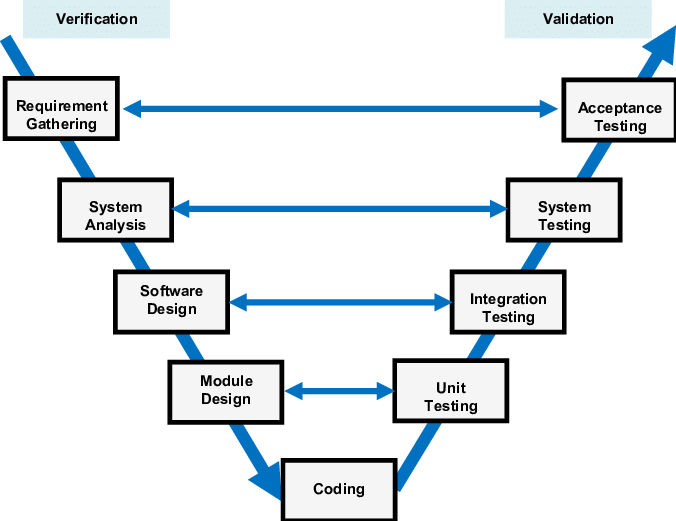
\includegraphics[width=0.75\textwidth]{./images/v_model.png}
    \caption{Illustration of the v-model process.}
    \label{fig:v-model-process}
\end{figure}

\newpage
\bibliographystyle{IEEEtran}
\bibliography{../../refs/References}

\newpage
\section*{Appendix --- Reflection}

The purpose of reflection questions is to give you a chance to assess your own
learning and that of your group as a whole, and to find ways to improve in the
future. Reflection is an important part of the learning process.  Reflection is
also an essential component of a successful software development process.  

Reflections are most interesting and useful when they're honest, even if the
stories they tell are imperfect. You will be marked based on your depth of
thought and analysis, and not based on the content of the reflections
themselves. Thus, for full marks we encourage you to answer openly and honestly
and to avoid simply writing ``what you think the evaluator wants to hear.''

Please answer the following questions.  Some questions can be answered on the
team level, but where appropriate, each team member should write their own
response:


Questions 3 and 5 are answered as a team.

\begin{enumerate}
  \item What went well while writing this deliverable? 

  \textbf{Kalp:} I think what went really well during the writing of the SRS
  document was the frequent in-person work sessions. We were all able to sit
  together in a room, quickly review each other's work, make changes, discuss
  unclear assignments, and so on. This process, compared to the individual
  writeup and review process we used earlier, was much more efficient and
  effective, especially since this document was very interdependet (goals
  section for example having content related to the requirements section).
  
  \textbf{Nirmal Chaudhari:} Coming up with the schedule and milestone for this
  project was relatively easy for the elicitation and documentation stages since
  it was basically just a recap and coherent with what we just went through.
  Moreover, since our team had come up with the list of focus areas in advance,
  coming up with team roles and added responsibilities was relatively easy as
  well. 
  
  \textbf{Sathurshan:} In this deliverable, the team effectively collaborated on
  specific sections, allowing us to provide constructive feedback and
  iteratively refine our requirements during the initial write-up. This process
  helped align our goals for the system and provided a clearer understanding of
  what needed to be achieved.

  \textbf{Omar}: Throughout the deliverable writing process, the team
  communicated effectively and responded to feedback on the pull requests in a
  timely manner. This allowed us to rapidly iterate on the document. Since
  everyone brings an equal level of commitment and enthusiasm to the project, it
  made the collaboration process smooth and enjoyable.

  \textbf{Jay:} Building on our earlier deliverables made the writing process 
  much smoother. Having already defined the problem scope and development plan 
  gave us a solid foundation to work from, so translating those ideas into 
  detailed requirements felt natural. The structured template also helped keep 
  everything organized, making it easier to ensure completeness across all 
  sections. 

  \item What pain points did you experience during this deliverable, and how did
  you resolve them?

  \textbf{Kalp:} I think the main pain point was the way that we divided up the
  work on the document since many of the sections were dependent on each other.
  This often lead to some people on the team waiting for others to finish their
  section before they could start their own so that there wasn't conflicting
  information or text in the document. This process was slighly improved with
  the frequent in-person work sessions, but it was still a pain point.
  
  \textbf{Nirmal Chaudhari:} While working on the environment section, intially
  coming up with the list of components in the environment the system will have
  to interact with as difficult. This is because of the ambuguity that initially
  existed with what we can consider the "environment" for this system. This
  unclearity was resolved by coming up with a very high level use-case scenario
  of what a typical person would be interacting with when using the device.
  \textbf{Sathurshan:} Many sections were dependent on others being completed
  first, which blocked some of the writing process. With the granted extension,
  several sections were delayed, leading to a time crunch toward the end. To
  address this, the team organized multiple collaborative work sessions to work
  on the SRS document together. This allowed us to exchange ideas in real time,
  resolve blockers quickly, and progress in parallel. Moving forward, during the
  project planning stage, the team should prioritize dependency related issues
  and set internal deadlines to ensure smoother progress.

  \textbf{Omar}: There was some friction when it came to sections that relied on
  other sections being completed first. However, the team was able to work
  through these issues by holding several in-person and virtual meetings to
  discuss the document and make progress together. This allowed us to quickly
  resolve any blockers and ensure that everyone was on the same page.

  \textbf{Jay:} Striking the right balance between technical precision and 
  readability was challenging. Some sections needed enough detail to be 
  actionable, but too much made them hard to follow. We addressed this by 
  reviewing each other's sections and providing feedback on clarity, which 
  helped us converge on a consistent level of detail throughout the document. 

  \item How many of your requirements were inspired by speaking to your
  client(s) or their proxies (e.g. your peers, stakeholders, potential users)?

  A lot of the requirements related to focus areas defined in our SRS document
  were inspired by our project supervisor. He gave great insight into what major
  components need to be researched for this system to work. For example, he went
  over the requirement of needing 4 ADC converters in our microprocessor to
  retrieve synchronized audio input across all 4 microphones. If he didn't give
  this insight early on, the team would have been stuck in the later stages on
  the project with a microprocessor that will not work well for this system.
  Furthermore, he gave good information of how the team can go about using
  Independent Component Analysis to seperate audio into sources. He also
  mentioned we shouldn't use deep machine learning models for audio
  classification, since they won't be able to run on the microprocessor well. 

  
  \item Which of the courses you have taken, or are currently taking, will help
  your team to be successful with your capstone project.

  \textbf{Nirmal Chaudhari: } For this project the three courses I think will
  enable us to be the most successful are: Signals \& Systems, Requirements
  Engineering and Software Design 2. Signals \& Systems was important since the
  entire project revolves around processing and analyzing audio signals in the
  frequency domain. Requirements Engineering is important in helping us figure
  out our requirements and ensuring throughout the entire process that what we
  are building is the right thing. And Software Design 2 is useful in helping us
  implement best practices into the project, thus making it sustainable in the
  future.

  \textbf{Sathurshan:} 3MX3: signal processing, 2GA3: computer hardware
  architecture. 3RA3: software requirements, 2DA4: software design, 3A04:
  software architecture, 3S03: software testing.

  \textbf{Omar}: The courses that will help us the most with this project are:
  Signals and Systems (3MX3) - This course provides a solid foundation in signal
  processing, which is crucial for our project focused on audio signal analysis.
  Concurrent Programming (3BB4) - This course teaches us the core principles of
  concurrent programming which will be essential for implementing real-time
  processing on our microcontroller.

  \textbf{Kalp:} The courses that will probably help us the most for this
  project are 3MX3 (Signals \& Systems with Dr. Mohrenschildt). This course
  taught us many of the signal processing algorithms for that we will likely
  need to apply during our audio analysis for the system. Another good course
  would be 3A04 (Software Architecture) that taught us how to design and
  implement large scale software systems which will be important for our project
  as we we will be designing many modular components that work together. The
  planning techniques from the course, specifically, will be very useful.

  \textbf{Jay:} 3MX3 (Signals \& Systems) is definitely critical for 
  understanding audio processing and frequency analysis. Beyond that, 
  3BB4 (Concurrent Systems) will be valuable for managing real-time 
  constraints on the microcontroller, and 2GA3 (Computer Architecture) 
  will help us optimize performance on embedded hardware. The software 
  engineering courses like 3RA3 and 3S03 are also important for ensuring 
  we build a reliable, well-tested system.

  \item What knowledge and skills will the team collectively need to acquire to
  successfully complete this capstone project?  Examples of possible knowledge
  to acquire include domain specific knowledge from the domain of your
  application, or software engineering knowledge, mechatronics knowledge or
  computer science knowledge.  Skills may be related to technology, or writing,
  or presentation, or team management, etc.  You should look to identify at
  least one item for each team member.

  Each memmber of the team requires the following qualfiications as contributing
  developers to the team.

  \begin{itemize}
    \item Embedded software development.
    \item Strong software design for features being implemented on any
    microcontroller platform. 
    \item Strong testing skills.
    \item Strong debugging skills. 
  \end{itemize}

  In addition to this, since each team member is a focus area expert, they
  require the following skills and competencies to carry out that role.

  \begin{itemize}\setlength\itemsep{4pt}\setlength{\leftmargini}{2em}
    \item Look through research articles, and technical evaluations to come up
    with feasibile approaches for proposed methods. 
    \item Collaborate with other team members to discuss findings. 
    \item Maintain clear and organized documentation of sources and proposed
    methods. 
    \item Ensure that all research and implementation choices align with project
     objectives, timeline and budgeting costs. 
    \item Based on the confirmed approach, complete the full implementation of
    that focus in the system. 
    \item After implementation, create test cases that cover's the main
    functionality of the feature in that focus area. 
    \item Configure github pipeline to run those tests on every PR and merge
    into a feature branch. 
  \end{itemize}


  \item For each of the knowledge areas and skills identified in the previous
  question, what are at least two approaches to acquiring the knowledge or
  mastering the skill?  Of the identified approaches, which will each team
  member pursue, and why did they make this choice?

  \textbf{Kalp:} I think the main focus for knowledge areas to explore has to be
  around embedded software development and hardware integration. Since I've only
  done software development in industry before, I have experience developing, 
  testing, and debugging software, but have never explored the hardware side of
  the systems. 

  \textbf{Nirmal Chaudhari:} For embedded software development and strong
  software design, two approaches are available: (1) reviewing processor
  documentation and (2) practicing and test building small programs on the board
  to see how it targets key peripherals work. I will focus on the second
  approach since practical experience seems more important. For testing and
  debugging skills, the team can (1) study or use existing knowledge of
  frameworks and (2), conduct peer reviews with other members on the team. For
  this I would prefer the second approach since working with the team on real
  bugs would help me grow as a developer to see how others resolve bugs. For
  research and technical evaluation, the knowledge can be gained by (1) reading
  research papers existing in the focus area and (2) contacting domain experts
  like mvm for insights. I plan to start with the first option, since academic
  resources provides structure that can be referenced to later on.
 
  \textbf{Sathurshan:} I plan to focus on gaining knowledge in embedded software
  development, as it is something I want to specialize in the next few years.

  \textbf{Omar}: I believe the best way to learn any skill is by doing it and
  struggling through problems. Each microcontroller platform has its own quirks
  and tools. I plan to gain practical experience by developing smaller projects
  on the STM32 platform, which will help me understand its architecture. Each
  problem in our project can be subdivided into smaller projects, which will
  help me learn as I go. Additionally, I will refer to the STM32 documentation
  and online tutorials to supplement my learning.

  \textbf{Jay:} I'll be focusing on Independent Component Analysis (ICA) for 
  audio source separation. Two main approaches are: (1) implementing ICA 
  algorithms from research papers and testing them with sample audio data, 
  and (2) prototyping directly on the hardware with real microphone input. 
  I'll start with the first approach since it lets me validate the core 
  algorithms quickly without hardware dependencies, then transition to 
  hardware testing once we have a stable foundation. I'll also lean on our 
  supervisor's expertise to guide algorithm selection and avoid overly 
  complex solutions.

\end{enumerate}


\end{document}